\section{Date: 2026-07-11}
\noindent \textbf{Series ID: CIS2026000000000I} 

\noindent This series is titled Employment Cost Index: Wages and salaries for Private industry workers in Education and health services and has a frequency of Quarterly. The units are Index Dec 2005=100 and the seasonal adjustment is Seasonally Adjusted.The observation start date is 2001-01-01 and the observation end date is 2026-01-01.The popularity of this series is 1. \\ 

\noindent \textbf{Series ID: T4245MM157NCEN} 

\noindent This series is titled Merchant Wholesalers, Except Manufacturers' Sales Branches and Offices: Nondurable Goods: Farm Product Raw Materials Inventories and has a frequency of Monthly, End of Month. The units are Percent and the seasonal adjustment is Not Seasonally Adjusted.The observation start date is 1992-02-01 and the observation end date is 2026-05-01.The popularity of this series is 2. \\ 

\subsection{Regression Tables and Plots}
\begin{center}
\begin{tabular}{lclc}
\toprule
\textbf{Dep. Variable:}                 & value\_fred\_T4245MM157NCEN & \textbf{  R-squared:         } &     0.005   \\
\textbf{Model:}                         &             OLS             & \textbf{  Adj. R-squared:    } &    -0.006   \\
\textbf{Method:}                        &        Least Squares        & \textbf{  F-statistic:       } &    0.4526   \\
\textbf{Date:}                          &       Sat, 11 Jul 2026      & \textbf{  Prob (F-statistic):} &    0.503    \\
\textbf{Time:}                          &           12:45:55          & \textbf{  Log-Likelihood:    } &   -466.08   \\
\textbf{No. Observations:}              &               101           & \textbf{  AIC:               } &     936.2   \\
\textbf{Df Residuals:}                  &                99           & \textbf{  BIC:               } &     941.4   \\
\textbf{Df Model:}                      &                 1           & \textbf{                     } &             \\
\textbf{Covariance Type:}               &          nonrobust          & \textbf{                     } &             \\
\bottomrule
\end{tabular}
\begin{tabular}{lcccccc}
                                        & \textbf{coef} & \textbf{std err} & \textbf{t} & \textbf{P$> |$t$|$} & \textbf{[0.025} & \textbf{0.975]}  \\
\midrule
\textbf{const}                          &      -0.7397  &       12.906     &    -0.057  &         0.954        &      -26.348    &       24.869     \\
\textbf{value\_fred\_CIS2026000000000I} &       0.0692  &        0.103     &     0.673  &         0.503        &       -0.135    &        0.273     \\
\bottomrule
\end{tabular}
\begin{tabular}{lclc}
\textbf{Omnibus:}       & 20.134 & \textbf{  Durbin-Watson:     } &    2.400  \\
\textbf{Prob(Omnibus):} &  0.000 & \textbf{  Jarque-Bera (JB):  } &   25.776  \\
\textbf{Skew:}          &  1.229 & \textbf{  Prob(JB):          } & 2.53e-06  \\
\textbf{Kurtosis:}      &  3.281 & \textbf{  Cond. No.          } &     660.  \\
\bottomrule
\end{tabular}
%\caption{OLS Regression Results}
\end{center}

Notes: \newline
 [1] Standard Errors assume that the covariance matrix of the errors is correctly specified.

\begin{figure}
\centering
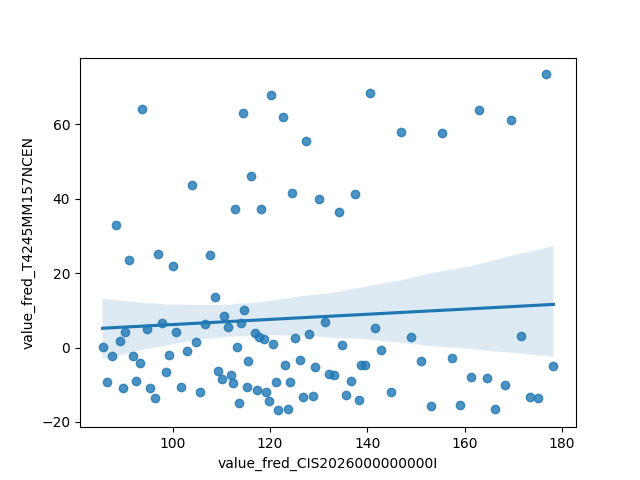
\includegraphics[scale = 0.9]{plots/plot_2026-07-11.png}
\caption{Regression Plot for 2026-07-11}
\end{figure}
\newpage
